% !TEX root = ../Coherence.tex

\section{Categorical coherence} 
\label{s:catoperads}
 
\subsection{Basic definitions}

Throughout this section we consider structures without units.
Unless otherwise stated, the adjective "non-unital" will be implicitly assumed. 

\begin{definition} 
\label{def:catoperad}
A \emph{categorified non-symmetric operad} $\mathcal{P}$ is a collection $\left\{  \mathcal{P}(n)  \right\}_{n\in \mathbb{N}}$ of small categories equipped with bifunctors  
$$ \begin{array}{clll}
\circ_i&\colon& \mathcal{P}(n) \times
                    \mathcal{P}(k)
                    \longrightarrow \mathcal{P}(n+k-1) \ ,
                    & \text{for}\ 1 \leq i \leq n \ ,
\end{array}  $$
and for each $\kappa \in \mathcal{P}(m)$,  $\mu \in \mathcal{P}(n)$, $\nu \in \mathcal{P}(k)$, $1 \leq i \leq m$, $1 \leq j \leq n$ natural isomorphisms 
$$ \begin{array}{clll}
    \beta_{\kappa,\mu,\nu}&\colon& 
    (\kappa \circ_i \mu) \circ_{j+i-1} \nu  \overset{\cong}{\longrightarrow} \kappa \circ_i (\mu \circ_j \nu) \ , &  \\
    \theta_{\kappa,\nu,\mu}&\colon& 
    (\kappa \circ_i \nu) \circ_{j+k-1} \mu 
    \overset{\cong}{\longrightarrow} (\kappa \circ_j \mu) \circ_i \nu \ , & \text{when}\ i < j \ , 
\end{array}  $$
such that the following diagrams commute: the pentagonal \\
\resizebox{\linewidth}{!}{
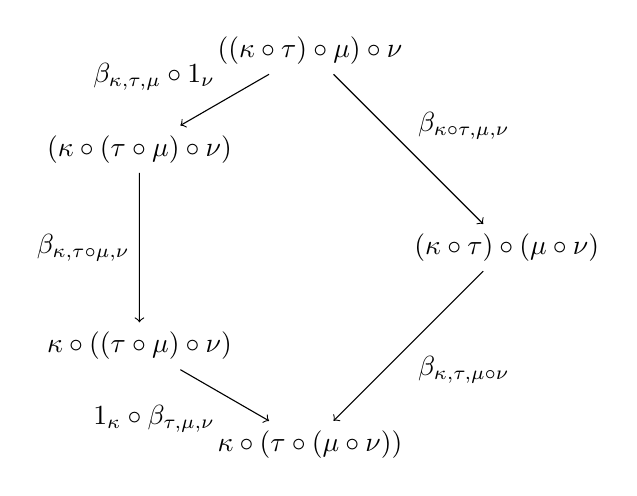
\begin{tikzpicture}[scale=2.5]
    \node (P1) at (0,1) {$((\kappa\circ\tau)\circ\mu)\circ\nu$};
    \node (P2) at (-0.866,0.5) {$(\kappa\circ(\tau\circ\mu)\circ\nu)$};
    \node (P3) at (-0.866,-0.5) {$\kappa\circ((\tau\circ\mu)\circ\nu)$};
    \node (P4) at (0,-1) {$\kappa\circ(\tau\circ(\mu\circ\nu))$};
    \node (P5) at (1,0) {$(\kappa\circ\tau)\circ(\mu\circ\nu)$} ;
    \draw[->] (P1)--(P2) node[midway,above left] {$\beta_{\kappa,\tau,\mu}\circ 1_\nu$};
    \draw[->] (P2)--(P3) node[midway,left] {$\beta_{\kappa,\tau\circ\mu,\nu}$};
    \draw[->] (P3)--(P4) node[midway,below left] {$1_\kappa \circ \beta_{\tau,\mu,\nu}$};
    \draw[->] (P1)--(P5) node[midway,above right] {$\beta_{\kappa\circ\tau,\mu,\nu}$};
    \draw[->] (P5)--(P4) node[midway,below right] {$\beta_{\kappa,\tau,\mu\circ\nu}$};
\end{tikzpicture} \quad 
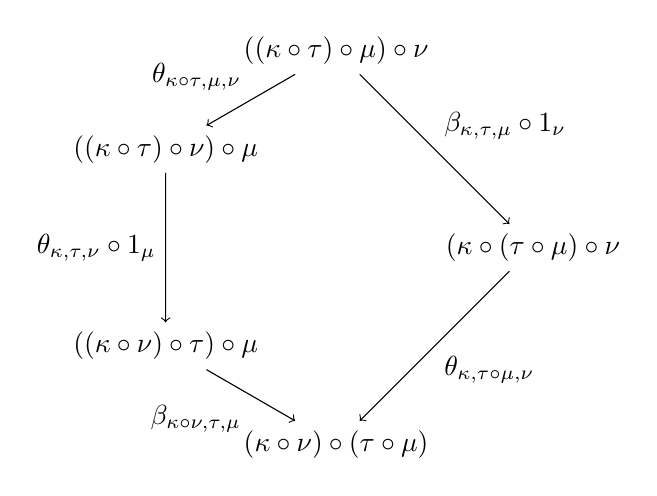
\begin{tikzpicture}[scale=2.5]
    \node (P1) at (0,1) {$((\kappa\circ\tau)\circ\mu)\circ\nu$};
    \node (P2) at (-0.866,0.5) {$((\kappa\circ\tau)\circ\nu)\circ\mu$};
    \node (P3) at (-0.866,-0.5) {$((\kappa\circ\nu)\circ\tau)\circ\mu$};
    \node (P4) at (0,-1) {$(\kappa\circ\nu)\circ(\tau\circ\mu)$};
    \node (P5) at (1,0) {$(\kappa\circ(\tau\circ\mu)\circ\nu$} ;
    \draw[->] (P1)--(P2) node[midway,above left] {$\theta_{\kappa\circ\tau,\mu,\nu}$};
    \draw[->] (P2)--(P3) node[midway,left] {$\theta_{\kappa,\tau,\nu}\circ 1_\mu$};
    \draw[->] (P3)--(P4) node[midway,below left] {$\beta_{\kappa\circ\nu,\tau,\mu}$};
    \draw[->] (P1)--(P5) node[midway,above right] {$\beta_{\kappa,\tau,\mu}\circ 1_\nu$};
    \draw[->] (P5)--(P4) node[midway,below right] {$\theta_{\kappa,\tau\circ\mu,\nu}$};
\end{tikzpicture} \quad 
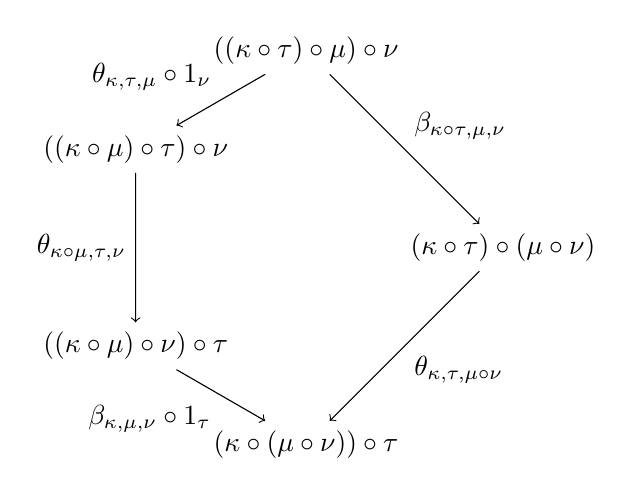
\begin{tikzpicture}[scale=2.5]
    \node (P1) at (0,1) {$((\kappa\circ\tau)\circ\mu)\circ\nu$};
    \node (P2) at (-0.866,0.5) {$((\kappa\circ\mu)\circ\tau)\circ\nu$};
    \node (P3) at (-0.866,-0.5) {$((\kappa\circ\mu)\circ\nu)\circ\tau$};
    \node (P4) at (0,-1) {$(\kappa\circ(\mu\circ\nu))\circ\tau$};
    \node (P5) at (1,0) {$(\kappa\circ\tau)\circ(\mu\circ\nu)$} ;
    \draw[->] (P1)--(P2) node[midway,above left] {$\theta_{\kappa,\tau,\mu}\circ 1_\nu$};
    \draw[->] (P2)--(P3) node[midway,left] {$\theta_{\kappa\circ\mu,\tau,\nu}$};
    \draw[->] (P3)--(P4) node[midway,below left] {$\beta_{\kappa,\mu,\nu}\circ 1_\tau$};
    \draw[->] (P1)--(P5) node[midway,above right] {$\beta_{\kappa\circ\tau,\mu,\nu}$};
    \draw[->] (P5)--(P4) node[midway,below right] {$\theta_{\kappa,\tau,\mu\circ\nu}$};
\end{tikzpicture} } \\
and hexagonal identities \\
\begin{center}
\resizebox{0.8\linewidth}{!}{
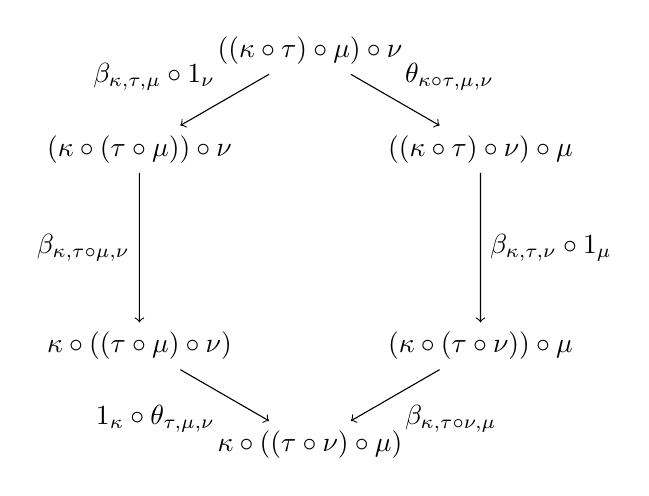
\begin{tikzpicture}[scale=2.5]
    \node (P1) at (0,1) {$((\kappa\circ\tau)\circ\mu)\circ\nu$};
    \node (P2) at (-0.866,0.5) {$(\kappa\circ(\tau\circ\mu))\circ\nu$};
    \node (P3) at (-0.866,-0.5) {$\kappa\circ((\tau\circ\mu)\circ\nu)$};
    \node (P4) at (0,-1) {$\kappa\circ((\tau\circ\nu)\circ\mu)$};
    \node (P5) at (0.866,0.5) {$((\kappa\circ\tau)\circ\nu)\circ\mu$} ;
    \node (P6) at (0.866,-0.5) {$(\kappa\circ(\tau\circ\nu))\circ\mu$};
    \draw[->] (P1)--(P2) node[midway,above left] {$\beta_{\kappa,\tau,\mu}\circ 1_\nu$};
    \draw[->] (P2)--(P3) node[midway,left] {$\beta_{\kappa,\tau\circ\mu,\nu}$};
    \draw[->] (P3)--(P4) node[midway,below left] {$1_\kappa \circ \theta_{\tau,\mu,\nu}$};
    \draw[->] (P1)--(P5) node[midway,above right] {$\theta_{\kappa\circ\tau,\mu,\nu}$};
    \draw[->] (P5)--(P6) node[midway,right] {$\beta_{\kappa,\tau,\nu}\circ 1_\mu$};
    \draw[->] (P6)--(P4) node[midway,below right] {$\beta_{\kappa,\tau\circ\nu,\mu}$};
\end{tikzpicture} \quad \quad
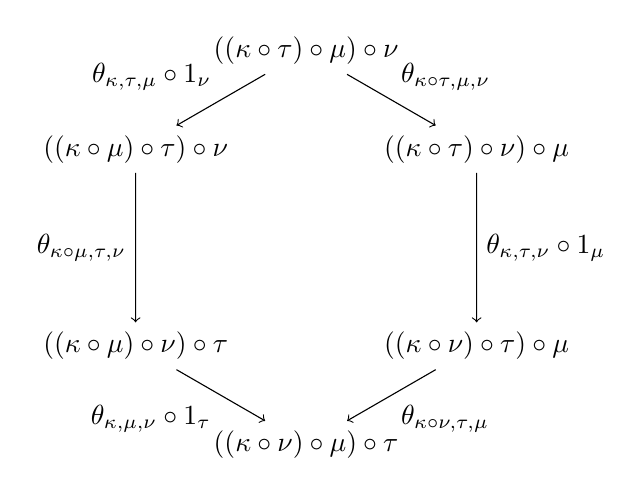
\begin{tikzpicture}[scale=2.5]
    \node (P1) at (0,1) {$((\kappa\circ\tau)\circ\mu)\circ\nu$};
    \node (P2) at (-0.866,0.5) {$((\kappa\circ\mu)\circ\tau)\circ\nu$};
    \node (P3) at (-0.866,-0.5) {$((\kappa\circ\mu)\circ\nu)\circ\tau$};
    \node (P4) at (0,-1) {$((\kappa\circ\nu)\circ\mu)\circ\tau$};
    \node (P5) at (0.866,0.5) {$((\kappa\circ\tau)\circ\nu)\circ\mu$} ;
    \node (P6) at (0.866,-0.5) {$((\kappa\circ\nu)\circ\tau)\circ\mu$};
    \draw[->] (P1)--(P2) node[midway,above left] {$\theta_{\kappa,\tau,\mu}\circ 1_\nu$};
    \draw[->] (P2)--(P3) node[midway,left] {$\theta_{\kappa\circ\mu,\tau,\nu}$};
    \draw[->] (P3)--(P4) node[midway,below left] {$\theta_{\kappa,\mu,\nu}\circ 1_\tau$};
    \draw[->] (P1)--(P5) node[midway,above right] {$\theta_{\kappa\circ\tau,\mu,\nu}$};
    \draw[->] (P5)--(P6) node[midway,right] {$\theta_{\kappa,\tau,\nu}\circ 1_\mu$};
    \draw[->] (P6)--(P4) node[midway,below right] {$\theta_{\kappa\circ\nu,\tau,\mu}$};
\end{tikzpicture}  } \quad \ .
\end{center}
\end{definition}
The diagrams above hold for all instances of composable $\beta$ and $\theta$; these depend on the indices $i,j,k$, which are omitted for the sake of readability. 
Observe that a categorified non-symmetric operad concentrated in arity $1$ is a non-symmetric monoidal category.

In \cref{def:catoperad} above, one can think about the objects of $\mathcal{P}(n)$ as operations with $n$ inputs and one output, and represent them by planar corollas. 
The $\circ_i$-isomorphisms then correspond to composition of these operations, or grafting of planar trees.
From this perspective, coherence diagrams stand for the operadic parallel and sequential associativity axioms, and there is one such diagram for every planar tree with four vertices. 

\begin{rem}
\label{rem:DPLA}
K. Do{\v s}en and Z. Petri{\'c} introduce in \cite[Section 12]{DP15} the notion of weak Cat-operad.
Despite looking different at first sight, the two notions are in fact equivalent.
The crucial observation is the following: the $\theta$-isomorphisms of Do{\v s}en--Petri{\'c} comprise both the isomorphisms~$\theta$ in \cref{def:catoperad} and their inverses $\theta^{-1}$.
Therefore, there are only two pentagonal coherence diagrams in the definition of a weak Cat-operad, the equations ($\beta$ $pent_e$) and ($\beta\theta 2_e$) of \cite[Section 9]{DP15}.
The set of diagrams of the form ($\beta$ $pent_e$) is the same as the set of diagrams which arises from the first pentagon in \cref{def:catoperad}, while the set of diagrams of the form ($\beta\theta 2_e$) is partitioned into the sets of diagrams which arise from the second and third pentagons in \cref{def:catoperad}.
\end{rem}

\begin{definition}
    A \emph{strong morphism of categorified non-symmetric operads} $F: \mathcal{P} \to \mathcal{Q}$ is a collection of functors $F_n : \mathcal{P}(n) \to \mathcal{Q}(n)$ together with natural isomorphisms $\gamma_{\kappa,\mu}: F_{m-1+n}(\kappa \circ_i \mu) \overset{\cong}{\longrightarrow} F_m(\kappa) \circ_i F_n(\mu)$ such that the following diagrams commute:
    \begin{center}
    \resizebox{0.8\linewidth}{!}{
    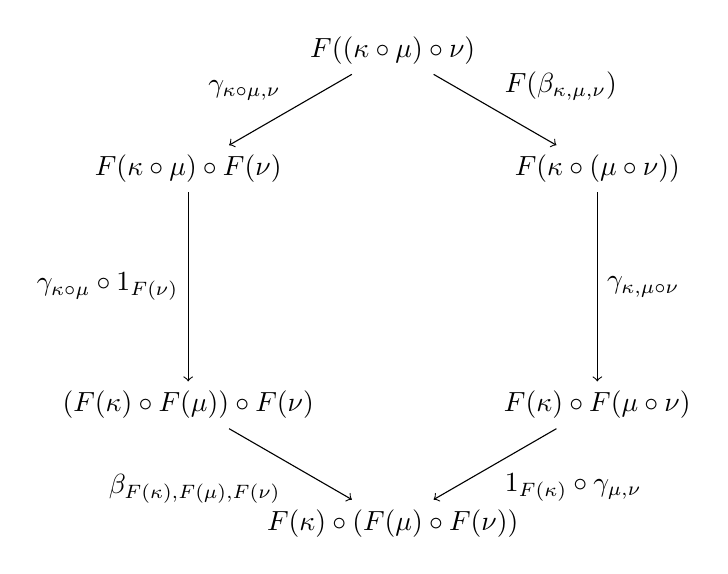
\begin{tikzpicture}[scale=3]
        \node (P1) at (0,1) {$F((\kappa\circ\mu)\circ\nu)$};
        \node (P2) at (-0.866,0.5) {$F(\kappa\circ\mu)\circ F(\nu)$};
        \node (P3) at (-0.866,-0.5) {$(F(\kappa)\circ F(\mu))\circ F(\nu)$};
        \node (P4) at (0,-1) {$F(\kappa)\circ(F(\mu)\circ F(\nu))$};
        \node (P5) at (0.866,0.5) {$F(\kappa\circ(\mu\circ\nu))$} ;
        \node (P6) at (0.866,-0.5) {$F(\kappa)\circ F(\mu\circ\nu)$};
        \draw[->] (P1)--(P2) node[midway,above left] {$\gamma_{\kappa\circ\mu,\nu}$};
        \draw[->] (P2)--(P3) node[midway,left] {$\gamma_{\kappa\circ\mu}\circ 1_{F(\nu)}$};
        \draw[->] (P3)--(P4) node[midway,below left] {$\beta_{F(\kappa),F(\mu),F(\nu)}$};
        \draw[->] (P1)--(P5) node[midway,above right] {$F(\beta_{\kappa,\mu,\nu})$};
        \draw[->] (P5)--(P6) node[midway,right] {$\gamma_{\kappa,\mu\circ\nu}$};
        \draw[->] (P6)--(P4) node[midway,below right] {$1_{F(\kappa)}\circ\gamma_{\mu,\nu}$};
    \end{tikzpicture}  \quad \quad
    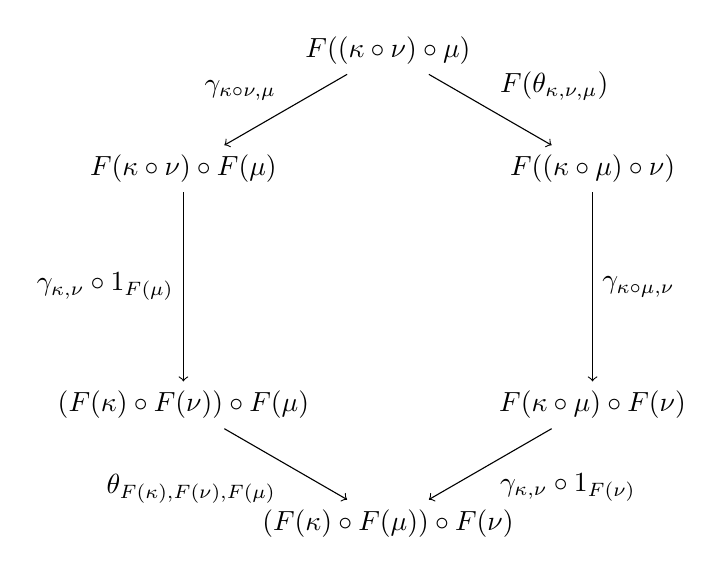
\begin{tikzpicture}[scale=3]
        \node (P1) at (0,1) {$F((\kappa\circ\nu)\circ\mu)$};
        \node (P2) at (-0.866,0.5) {$F(\kappa\circ\nu)\circ F(\mu)$};
        \node (P3) at (-0.866,-0.5) {$(F(\kappa)\circ F(\nu))\circ F(\mu)$};
        \node (P4) at (0,-1) {$(F(\kappa)\circ F(\mu))\circ F(\nu)$};
        \node (P5) at (0.866,0.5) {$F((\kappa\circ\mu)\circ\nu)$} ;
        \node (P6) at (0.866,-0.5) {$F(\kappa\circ\mu)\circ F(\nu)$};
        \draw[->] (P1)--(P2) node[midway,above left] {$\gamma_{\kappa\circ\nu,\mu}$};
        \draw[->] (P2)--(P3) node[midway,left] {$\gamma_{\kappa,\nu}\circ 1_{F(\mu)}$};
        \draw[->] (P3)--(P4) node[midway,below left] {$\theta_{F(\kappa),F(\nu),F(\mu)}$};
        \draw[->] (P1)--(P5) node[midway,above right] {$F(\theta_{\kappa,\nu,\mu})$};
        \draw[->] (P5)--(P6) node[midway,right] {$\gamma_{\kappa\circ\mu,\nu}$};
        \draw[->] (P6)--(P4) node[midway,below right] {$\gamma_{\kappa,\nu}\circ 1_{F(\nu)}$};
    \end{tikzpicture}  } \quad \ .
\end{center}
    It is said to be \emph{strict} if the natural isomorphisms are identities. 
\end{definition}

Once again, the diagrams above hold for all instances of $\beta$ and $\theta$ arrows, and we have omitted the $(i,j,k)$-indices for readability. 
Observe that a strong (resp. strict) morphism between categorified non-symmetric operads concentrated in arity $1$ is a strong (resp. strict) monoidal functor between non-symmetric monoidal categories. 

\subsection{Coherence theorem}

We now aim at the coherence theorem for categorified non-symmetric operads.
We start from a family of sets $S=\{S_n\}_{n \geq 1}$.
Then, we build a syntax $\mathcal{S}$ with object terms $T=\{T_n\}_{n\geq 1}$ by the following rules:
\begin{enumerate}
    \item if $\kappa \in S_n$, then $\kappa$ is a term and $\kappa \in T_n$;
    \item if $\kappa \in T_m$ and $\mu \in T_n$ are terms and $1 \leq i \leq m$, then $\kappa \circ_i \mu$ is a term and $\kappa \circ_i \mu \in T_{m-1+n}$.
\end{enumerate}
Now we define a set $B$ of basic morphisms $1_t : t \to t$ for all terms $t\in T$, $\beta: (\kappa \circ_i \mu) \circ_{j+i-1} \nu \leftrightarrow \kappa \circ_i (\mu \circ_j \nu) : \beta^{-1}$ for every $\kappa \in T_m, \mu \in T_n, \nu \in T_k$ and $1 \leq i \leq m$ and $1 \leq j \leq n$, and $\theta: (\kappa \circ_i \nu) \circ_{j+\ari(\nu)-1} \mu \leftrightarrow (\kappa \circ_j \mu) \circ_i \nu : \theta^{-1}$ whenever $i<j$, and we define the morphism terms of our syntax by the following rules:
\begin{enumerate}
    \item if $\beta \in B$, then $\beta$ is a morphism term; 
    \item if $\phi_1: t_1 \to t_2$ and $\phi_2: t_2 \to t_3$ are morphism terms, then $\phi_2 \phi_1 : t_1 \to t_3$ is a morphism term;
    \item if $\phi_1 : t_1 \to t_2$ and $\phi_2 : t_3 \to t_4$ are morphism terms $t_1,t_2 \in T_n$ and $1 \leq i \leq n$, then $\phi_1 \circ_i \phi_2 : t_1 \circ_i t_3 \to t_2 \circ_i t_4$ is a morphism term. 
\end{enumerate}
This finishes the construction of our syntax. 
Observe that any morphism in our syntax can be written uniquely as a composite of morphisms made up of only one non-identity basic morphism. 

\begin{definition}
    We denote by $\mathcal{F}(S)$ the quotient of the syntax $\mathcal{S}$ by the axioms of categories, the axioms of bifunctors, and the coherence diagrams defining a categorified non-symmetric operad. 
\end{definition}

We obtain that $\mathcal{F}(S)$ is the free categorified non-symmetric operad on $S$. 
That is, for any categorified non-symmetric operad $\mathcal{P}$, and for family of functions $\rho_n : S_n \to \obj(\mathcal{P}(n))$, there is a unique strict morphism of non-symmetric categorified operads $[-]:\mathcal{F}(S) \to \mathcal{P}$ that extends $\rho=\{\rho_n\}_{n\geq 1}$. 

\begin{thm}[Coherence theorem]
\label{thm:coherence-operahedra}
    For any categorified non-symmetric operad $\mathcal{P}$, for any family of functions $\rho : S \to \obj(P)$, and for any two parallel morphisms $\phi_1,\phi_2: t_1 \to t_2$ in $\mathcal{F}(S)$, we have $[\phi_1]=[\phi_2]$.
\end{thm}

\begin{proof}
The morphisms of $\mathcal{F}(S)$ are in bijection with combinatorial paths on a family of polytopes called operahedra \cite[Section 2.1]{laplante-anfossiDiagonalOperahedra2022a}, see also \cite[Section 13]{DP15}, whose faces are in bijection with the set of all nestings on a planar tree. 
Two parallel morphisms in $\mathcal{F}(S)$ thus define two parallel combinatorial parths on some operahedron. 
Since an operahedron is simply connected, \cref{thm:top-coherence} implies that these two combinatorial paths are combinatorially homotopic. 
The result then follows from the fact that a $2$-face of an operahedron is exactly either a square (witnessing naturality), a pentagon or an hexagon (witnessing a coherence condition) as in \cref{def:catoperad} above.
\end{proof}
   
Following \cref{rem:DPLA}, we have that \cref{thm:coherence-operahedra} gives an alternative, more economical proof of coherence for weak Cat-operads \cite[Proposition 14.2]{DP15}. 
Restricting the theorem above to non-symmetric operads concentrated in arity $1$, the category $\mathcal{F}(S)$ becomes the free non-symmetric monoidal category on $S$, and we get the following corollary. 

\begin{corollary}[MacLane's coherence theorem]
\label{cor:MacLane}
    For any non-symmetric monoidal category $\mathcal{C}$, for any function $\rho : S \to \obj(\mathcal{C})$, and for any two parallel morphisms $\phi_1,\phi_2: t_1 \to t_2$ in $\mathcal{F}(S)$, we have $[\phi_1]=[\phi_2]$.
\end{corollary}

\begin{proof}
    The morphisms in $\mathcal{F}(S)$ are in bijection with combinatorial paths on the associahedra \cite{Stasheff63,CSZ15}, a subfamily of the operahedra associated to linear trees. 
    One checks easily that each $2$-face of an associahedron is either a square (witnessing naturality) or a pentagon (witnessing a coherence condition) of the type considered by MacLane \cite[Equation 3.5]{MacLane63}.
\end{proof}

One can use the exact same strategy to prove coherence theorems for 
\begin{itemize}
    \item \emph{symmetric} monoidal categories, using the family of permutoassociahedra \cite{kapranov1993,reinerCoxeterassociahedra1994}, and
    \item \emph{unital} non-symmetric monoidal categories, using the unital associahedra of F. Muro and A. Tonks \cite{muroUnitalAssociahedra2014}.
\end{itemize}
It is natural to ask if the construction of unital associahedra could be extended to the permutoassociahedra, in such a way as to provide a topological proof of coherence for unital symmetric monoidal categories. 
The question of the existence of these constructions at the operadic level (i.e. does there exist unital operahedra, symmetric operahedra, and unital symmetric operahedra?) is, to our knowledge, still open as well. 

\subsection{Further applications} 
\label{sec:further}
Another immediate application of \cref{thm:top-coherence} is the coherence of strong non-symmetric monoidal functors between non-symmetric monoidal categories \cite{epsteinFunctorsTensoredCategories1966}. 
The corresponding topological objects are in this case the family of multiplihedra \cite{Stasheff70,Forcey08}.
The generalization to strong morphisms between non-symmetric categorified operads also goes through, involving this time the family of multiploperahedra described at the end of the introduction in \cite{MazuirLA22}.

In the same spirit as in \cref{thm:coherence-operahedra}, one could obtain coherence results for categorifications of many operad-like structures, for instance the ones described in \cite{BMO20}: categorified modular operads, wheeled properads, and permutads (shuffle algebras), among others.
In order to treat cyclic and symmetric structures, one could take inspiration from the reduction process followed in \cite{curienCategorifiedCyclicOperads2020} for the case of cyclic symmetric categorified operads.

\subsection{Higher categories} 
\label{sec:higher}
\cref{thm:top-coherence} demonstrates that, in the case of monoidal categories, coherence is equivalent to the vanishing of the first homotopy groups of the associahedra. 
Since the associahedra are contractible, and therefore all their homotopy groups vanish, one could hope for a topological proof of higher dimensional coherence theorems.
Seeing a monoidal category as a bicategory with one object, one can ask about a coherence theorem for tricategories with one object. 
A first look at the diagrams in the beginning of \cite[Section 2]{gordonCoherenceTricategories1995} suggests that such a theorem should be at least related to the vanishing of the second homotopy groups of the associahedra.  
To formulate higher dimensional statements, one needs a good structure of pasting scheme on each associahedron, which is the subject of ongoing work \cite{AMMLA}.  

